 \chapter{Background and Related Work}
\label{chptr:concepts}

All systems that are designed based on the \abr{ETCS} specification must be safety-critical~\cite{OnBoardUnitSafetyTesting}. 
Introducing redundancy to safety-critical systems is a popular approach to ensure that faults inside the system do not lead to failures that affect the system's environment.
A system that can continue its intended work even in the presence of faults is said to be fault-tolerant~\cite{BarryFaultToleranceAnalysis}.
Redundancy can be achieved in multiple ways, some of which being adding additional resources (hardware redundancy), adding additional information or messages (information redundancy), or performing the same operation multiple times (time redundancy).
Although being one of the most often used redundancy techniques, the addition of hardware components, called replicas for redundant computation, leads to multiple results that need to be consolidated to a final system result.
Thus, the replicas need to communicate with each other and synchronize their results to act like a single unit in their environment.
A promising approach to cope with the communication overhead is \gls*{DDS}, a \gls*{DCPS} system, since it allows reliable and real-time communication~\cite{omgDDSspec}.
However, while hardware redundancy enhances a system's fault-tolerance, it also increases its costs and complexity.
\\

In the first section of this chapter, an introduction to \abr{ETCS} and its three levels is provided.
Afterward, an overview about the \abr{DDS} standard and its concepts is exposed.
In the third section, terms, criteria, and concepts for evaluating the safety and reliability of redundant systems are described.
Then, different redundancy concepts are explained and weighted against each other regarding reliability, safety, and performance.
Finally, standards for building and designing safe and fault-tolerant systems are given, and related works that successfully applied \gls*{DCPS}-middleware in the railway context are shown.

\section{\glsentryfull{ETCS}}
In order to facilitate interoperability between national railway systems throughout Europe, the signaling and speed control system has been standardized by the European Union under the term of \abr{ERTMS}.
\abr{ETCS} defines the signaling and train control component of \abr{ERTMS}~\cite{ETCS26}.
As such, \abr{ETCS} defines concepts for monitoring a train's speed, calculating the permissible speed restrictions, and coordinating the collaboration between track-side components, such as \abr{ETCS} euro-balises and on-board systems.
Any train requires a \abr{MA} to be allowed to drive from one location to another.
Besides encoding a train's permission to move, a \abr{MA} also encodes information about the track's conditions, such as gradient profiles and speed limitation.
Any \abr{MA} is supplied by an external entity, called \abr{RBC}, via track-side components or via radio frequencies.
A system that is located on the operating train - called on-board unit - monitors compliance with the current \abr{MA}.
The track-side components, as well as the on-board unit, are standardized according to three different \abr{ETCS} levels.

\paragraph{\abr{ETCS} level one}
\abr{ETCS} level one is designed to build upon existing signaling systems.
\abrpl{MA}, as well as route data and the maximum allowed speed, are transmitted through fix positioned euro-balises.
Parallel to that, a breaking curve and the train's position are permanently calculated and compared to the \abr{MA}'s limitations by an on-board unit.

\paragraph{\abr{ETCS} level two}
For \abr{ETCS} level two, signaling and \abr{MA} data is transmitted via mobile communication channels from the \abr{RBC} and displayed to the driver.
The \abr{RBC} is a central unit that constantly collects and supervises train movements and track information.
Although each train observes its own position, it can come to inaccuracies, for example due to a faulty sensor calibration.
Hence, a train operating under \abr{ETCS} level two does not know its exact position but can only locate itself within a certain range.
This range is called \textit{confidence interval} and consists of an upper and lower limit of an area where the train's actual position lies.
In order for the on-board unit to determine a train's exact position, track-side balises are used.
Before the train starts its journey, the positions of the balises that it will encounter on its journey are provided during a phase called the linking phase.
Thus, when a train crosses a linked balise and receives the balise telegram, the on-board unit can reset the train's position to the balises position.

\paragraph{\abr{ETCS} level three}
Finally, in \abr{ETCS} level three, any track-side component is abolished and the entire communication takes place via radio signals.
This \abr{ETCS} level is not fully standardized yet.

\section{\glsentryfull{DDS}}

\begin{figure}[!hb]
	\centering
	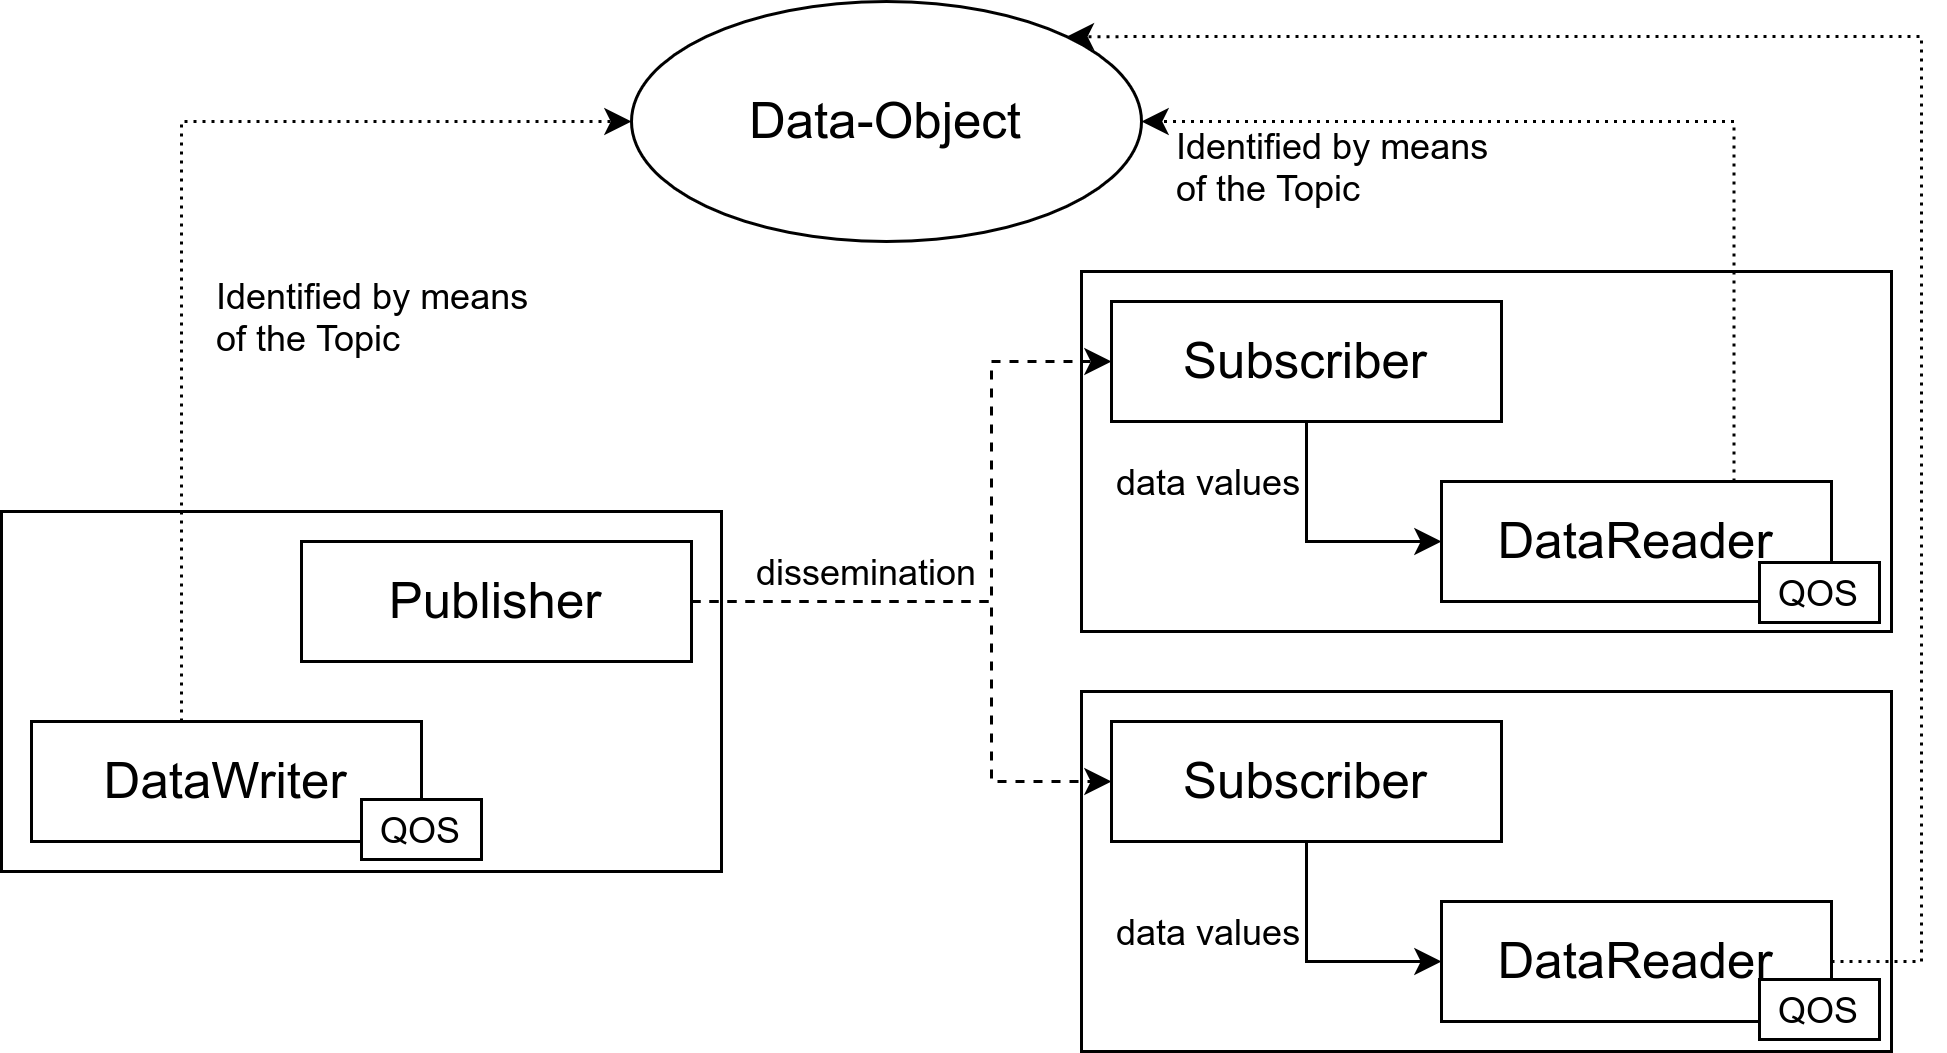
\includegraphics[width=0.8\linewidth]{images/DDSStructure}
	\caption{The \glsentryfull{DDS} is a data-centric communication model and follows the publish/subscribe pattern. The publishing and subscribing components do not communicate directly with each other but use topics to read and write data objects.}
	\label{fig:DDSStructure}
\end{figure}

\Gls*{DDS} is a \gls*{DCPS} model for machine-to-machine communication, that is specified by the \gls*{OMG}~\cite{omgDDSspec}.
It is stated that the model should, for practical use, be implemented as middleware in order to interface with the underlying \gls*{OS}.
The model follows a global data space concept and facilitates data exchange among entities based on type and content.
Central entities are \texttt{Publishers} and \texttt{Subscribers}, while data exchange is based on \texttt{Topics}.
A \texttt{Publisher} is used for sending data of different types.
In order to send expressly typed data, a \texttt{DataWriter} object is used, which acts as a typed interface to a \texttt{Publisher}.
On the other side, a \texttt{Subscriber} is used to receive data and make it accessible to the receiving application.
The equivalent of the \texttt{DataWriter} for the \texttt{Subscriber} is the \texttt{DataReader} object.
A \texttt{Topic} acts as the connecting element between publishing entities on the one side and subscribing entities on the other.
Any forecasting of when and how data is published to a \texttt{Topic} or received by a \texttt{Subscriber} is made possible through so-called \glspl*{QOS} policies.
This concept is illustrated in~\autoref{fig:DDSStructure}, which is based on the official \gls*{DDS} specification~\cite{omgDDSspec} and shows the information flow from the publishing to the subscribing side.

An application can either rely on the middleware to asynchronously notify it about the presence of new data through so-called \texttt{Listeners} or actively wait for new data by utilizing \texttt{WaitSets}.
A \texttt{WaitSet} can be attached with different \texttt{Conditions}, for example \texttt{ReadConditions}, and allows the application to wait until either one or more of the attached conditions are satisfied, or until the waiting times out.
Examples for conditions are \texttt{ReadCondition} and \texttt{QueryCondition}.
The \texttt{ReadCondition} object allows to name specific data samples and is met when the specified type of data is present in a \texttt{DataReader}.
A \texttt{QueryCondition} is a specified \texttt{ReadCondition} that further provides capabilities of filtering the data that is read through a \texttt{DataReader}.
\\

The usefulness of \gls*{DDS} for containerization technologies in automotive architectures has been studied by Kugele \etal~\cite{KugeleDataCentricForAuto}.
Although their findings are based on containerization technologies and are therefore not resilient for this work, Kugele \etal showed that the applicability of \gls*{DDS} with regards to safety, certification, and security depends on the actual implementation's characteristics.
Therefore, Vortex OpenSplice DDS is used throughout this thesis, which is developed and maintained by ADLINK.

The applicability of the \gls*{DDS}-standard and of Vortex OpenSplice \gls*{DDS} for safety-critical railway applications has been demonstrated by Schmidt and van't Hag~\cite{SchmidtMissionCriticalChallenges}.
Their findings show that OpenSplice \gls*{DDS}'s \gls*{QOS} policies allow predictable time and locality characteristics for data distribution.
Further, their work provides an overview about Vortex OpenSplice's \gls*{QOS} policies and features to ensure reliability, availability, data delivery, and resource usage.

\section{Techniques for Safety and Reliability Evaluation}
\label{sec:techniquesSafetyReliability}
In order to profoundly express and analyze redundancy techniques towards their safety, reliability, and fault-tolerance, the meaning of these characteristics needs to be defined.
\\

Reliability is, by IEEE 610.12-1990, defined as the ability of a system or component to perform its required function under stated conditions for a specified period of time~\cite{ieee610.12}.
A circumstance where a system deviates from its requirement is called a system failure.
A failure is preceded by a fault, which describes a static defect of a system~\cite{AmmannOffutt2016}.
When a fault becomes active, it manifests itself as an error, which marks an incorrect internal system state.
A failure occurs as soon as the error affects the system's environment.

\begin{definition}
A system or a system component failure is a state where its actual behavior deviates from its specified behavior.
\end{definition}

The definition of reliability used in this work is the following:

\begin{definition}
\label{def:reliability}
A system's reliability is a function of time that expresses the probability for the system to operate as specified at a time $t_1$, given that it was operating as specified at time $t | t \leq t_1$.
\end{definition}

In other words, reliability is a system's ability not to have any failure for a specific period of time.

A system's safety is associated with its reliability since it constitutes an extension of reliability~\cite{AvizienisDependability2001}.
In general, safety defines the absence of catastrophic failures of the system on its environment.
When non-catastrophic failures can be reliably detected and a safe state can be taken in case of failures, safety can be treated as reliability concerning catastrophic failures.
In other words, safety can be expressed as a system's probability not to experience any fault that would lead to a catastrophic failure in a specific period.

Based on these definitions, it can be conducted that a system's safety and reliability can only be finally assessed when the system's environment, the reliability of the system's components and the operations performed by the system are known.
In addition, the system's architecture and structure need to be acquainted.
Finally, in order to precisely evaluate a system's safety, possible faults and their consequences need to be known.
In order to be able to evaluate and compare different architectural patterns towards their safety characteristics, independently of the subsequently conducted operations, the definition of \texttt{intrinsic safety}, made by~\cite{BoulangerStandards}, is used in this work.

\begin{definition}
A system is said to be intrinsically safe if one can be certain that any failure of one or more components of that system will only result in its becoming more permissive.
In the railway context, a complete stoppage is generally the safest state.
\label{def:intrinsic_safety}
\end{definition}

This definition requires that measures are taken to assure the system's safety even in the presence of failures.
A system that provides the functionality to behave as specified even in the case of faults is said to be fault tolerant~\cite{AvizienisDependability2001}.
Fault tolerance is generally obtained through error detection, which allows the system to determine errors and enables it to mitigate resulting failures.
In the course of this thesis, the following definition is used for safety:

\begin{definition}
A system is said to be safe when the fault of the system or any of its components does not lead to a catastrophic failure.
\label{def:safety}
\end{definition}

Thus, to be considered secure, a distributed system must tolerate possible faults that could occur in distributed systems.
Flaviu Cristian has established the following five fault classes for distributed distributed systems~\cite{CristianFaultModel}:

\begin{enumerate}
\item \textbf{F1:} One or multiple components in the system crash (\textbf{crash fault}).
\item \textbf{F2:} One or multiple components fail to respond to an incoming request (\textbf{omission fault}).
\item \textbf{F3:} One or multiple components fail to produce an output within a certain time span (\textbf{timing fault}).
\item \textbf{F4:} One or multiple components produce a wrong result (\textbf{computation fault}).
\item \textbf{F5:} One or multiple components produce arbitrary responses at arbitrary times (\textbf{byzantine fault}).
\end{enumerate}

It applies, that all fault classes \textbf{Fx} are included in \textbf{Fy}, given that $y \geq x$.
In this thesis, the fault classes \textbf{F1} to \textbf{F4} are analyzed and byzantine faults are not covered.
\\

A necessary condition for a system to be safe is that the system is reliable.
One method of analyzing a system's reliability is through mathematical functions of time, for example the \texttt{exponential failure law}~\cite{GeffroyMotetDependableComputing}.
It describes a component's reliability as an exponential function on time.
\begin{equation}
R(t) = e^{-\lambda t}.
\label{eq:expFailureLaw}
\end{equation}
The parameter $\lambda$ is called the failure rate and encodes the probability of failures occurring in a specific time span, typically in an hour.
For the exponential failure law it is, mathematically, assumed that the components fail independently.
The independence of components might not always be the case in practice, as common core or power outage failures can affect multiple components at once.
However, the probability of failures affecting multiple components at once can be reduced by various techniques, such as using independent power supplies or diverse redundancy, the latter of which being discussed below.
\\

Among various theoretical techniques for evaluating a system's reliability, \textit{Markov chains} are one of the most commonly used~\cite{BarryFaultToleranceAnalysis}.
\textit{Markov chains} are a stochastic process that models the alterations of a system's state and probabilities for the system to transition into a specific state given that it was in a certain state~\cite{KemenyMarkovChains}.
Thereby, the next state only depends on the current state and is independent of all previous system modifications.

For safety analysis, each state models the system in one out of three conditions:
\begin{enumerate}
\item The system functions without having an error.
\item The system detects and successfully mitigates an error without leading to a failure
\item The system either not detects an error or does not recover from it, leading to a failure
\end{enumerate}

For the state transition probabilities, the exponential failure law~\autoref{eq:expFailureLaw}, with a constant failure rate $\lambda$, holds.

\begin{figure}[!hb]
	\centering
	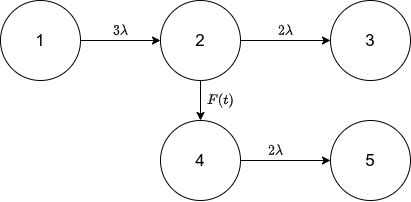
\includegraphics[width=0.8\linewidth]{images/TriplexSystemNASA}
	\caption{A reliability model for \glsentryfull{TMR} using Markov chains. In state (1), all three replicas are working. The transition from (1) to (2) shows the failure of any of the replicas. Because homogeneous components are used, they all have a failure rate of $\lambda$. The transition from (2) to (4) represents the identification of the faulty component, which succeeds which a probability of $F(t)$. The system is still operational in (4) because the fault identification allows the voter can distinguish a good result from a bad one. Therefore, the system would still be functional when another component fails (5) but not when another component fails without identifying faulty components (3).}
	\label{fig:NASATMR}
\end{figure}ha 

An example Markov chain for a system using three replicas is proposed by NASA and depicted in~\autoref{fig:NASATMR}~\cite{NASAMarkovChains}.
At state (1), assuming that the system is homogeneous redundant, the probability that one of the replicas fails is $3\lambda$.
In state (2), the system applies failure detection and mitigation procedures and has a chance of $F(t)$ for successful reconfiguration, which allows the system to continue its work.
However, there is still a change of $2\lambda$ that another component fails before the system detects and mitigates the first failure, which would lead to a system fault and render the entire system unsafe.
In state (4), there is again a $2\lambda$ change for one of the remaining components to fail, which would lead to a system failure.

As experiments have shown, a system's recovery time is not necessarily exponential~\cite{TheoryAndPracticeReliableSystem}.
Thus, it is expressed by $F(t)$, which is the probability that the system recovers within a time-span less than $t$.
In a diverse redundant system, each component failure is represented with an individual state.

\section{Redundancy Patterns}
\label{sec:redundancyPatterns}
Redundancy is a typically applied technique for handling and masking errors in a system and thereby enhancing a system's reliability~\cite{TanenbaumSteen07}.
Error masking is the concept of detecting and mitigating errors so that they do not become failures and affect the system's environment.
For redundancy, additional resources or information are added to a system that would not be required when errors were impossible to happen.
Barry Johnson defines redundancy in the following way~\cite{BarryFaultToleranceAnalysis}:
\begin{definition}
Redundancy implies the addition of information, resources, or time beyond what is needed for regular system operation.
It can take one of several forms, including hardware, software, information, and time redundancy.
\end{definition}

Each form of redundancy has its unique characteristics and patterns, which are presented in the following.

\subsection{Hardware Redundancy}
In hardware redundancy, additional replications of physical components are added to the system.
This typically increases the system's reliability by masking internal failures, but also increases the system's cost.
In general, a system's safety can be further improved when using components that are based on different internal components.
Using different components in redundancy patterns is called diverse redundancy while replicating the same components is called homogeneous redundancy~\cite{HomogeneousRedundancyOuzineb}.
Using diverse redundancy has the benefit of reducing the effect that common core errors have on a system's or component's safety.

Johnson subdivides hardware redundancy into two parts, namely passive and active redundancy.
In passive hardware redundancy, a voter or consensus algorithm is used to reduce the number of redundant outputs to a single output in order to prevent individual internal failures from propagating out of the system.
For active hardware redundancy, the system tries to detect and repair any internal failure, for example by replacing the faulty component.
While \gls*{MOON} systems are a typical example of passive hardware redundancy, standby redundancy is often used as an example of active hardware redundancy.

A voter can be realized in both software and hardware.
The benefits of software voters are that they typically cost less and are easier to develop because no special hardware is required.
However, software voters tend to operate slower.
The benefit of hardware voters is that they can operate faster and a minimal set of hardware needs to be approved, which reduces the time and cost expenses for approving the system.

Both types of voters have in common that they require time constraint synchronization with the replicas to collect their intermediate results, perform voting, and recognize failed or delayed redundant results.
Therefore, the individual replicas communicate their results to the voter, which collects the results, performs the voting, and generates a single system result.
The voting process facilitates the system to allow single replicas to produce wrong results without rendering the overall system result wrong.
In an active hardware redundant system - where the individual components are independent and communicate via a shared communication medium - the synchronization process is further impeded.
This is due to the impossibility of agreeing on values in asynchronous distributed systems with possibly faulty components~\cite{FLPProblemConsensus}.
Consequently, synchronizing the communication is required, which can be achieved through time constraints in the form of timeouts.
This can be, for example, achieved by starting a timer after a first replica sent its result or by letting the voter request the result from each replica.
In addition, an expired timeout can indicate crashed replicas or network partitions.

\paragraph{M-out-of-N Systems}
\begin{figure}[!hb]
	\centering
	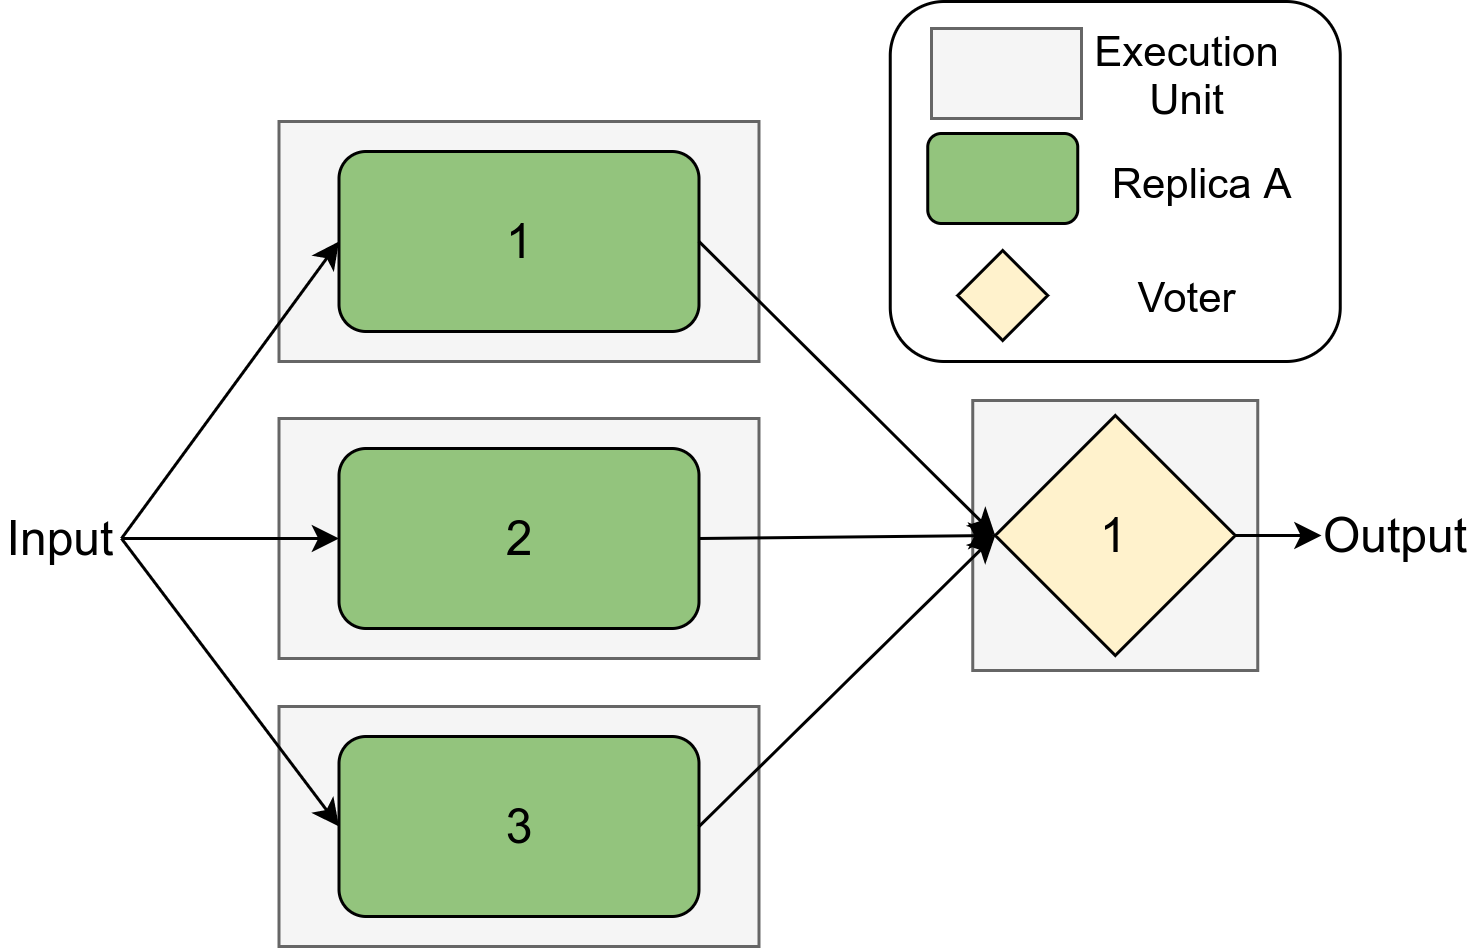
\includegraphics[width=0.8\linewidth]{images/Classical2OO3}
	\caption{Classical 3-out-of-2 redundancy, also known as \glsentryfull{TMR}. Three replicas are simultaneously reading and redundantly processing an input. A voter collects these redundant results and performs a majority voting to produce a final output.}
	\label{fig:Classical2OO3}
\end{figure}

One of the most common versions of \gls*{MOON} systems is \gls*{TMR} as shown in~\autoref{fig:Classical2OO3}.
In \gls*{TMR}, three replicas receive the same input and perform the same work in parallel.
A voter collects the individual outputs and reduces them to a single system output based on majority voting.
The system output must qualify the characteristic that at least two out of the three replicas agree on this output.
This allows the entire system to produce a correct output even in the presents of a faulty replica.
All replicas, as well as the voter, are running on individual execution units.

Instead of having one voter that decides about the final result, the calculations could be modularized and votings on intermediate results could be made.
Intermediate voting would have the benefit of masking intermediate faults and not letting them influence further calculations.
An example of how this could be achieved is depicted in~\autoref{fig:IntermediateVoting}.
\\

The biggest weakness of \gls*{TMR} is the voter because it marks a single point of failure.
Therefore, the voter's reliability in the system has to be high compared to the remaining replicas because the entire system's reliability cannot be higher than the voter's reliability.
Arifeen \etal propose a highly reliable hardware voter for making the voting process more reliable~\cite{ArifeenFaultTolerantTMR}.
An alternative to voters is a consensus algorithm, where all components, not only a single voter, are involved in deciding about the system's output value~\cite{lamport2001paxos}.
While not having a single point of failure anymore, consensus approaches typically introduce a communication overhead and lead to rigid configurations~\cite{GamerIncreasingMOON}.

\begin{figure}[!hb]
	\centering
	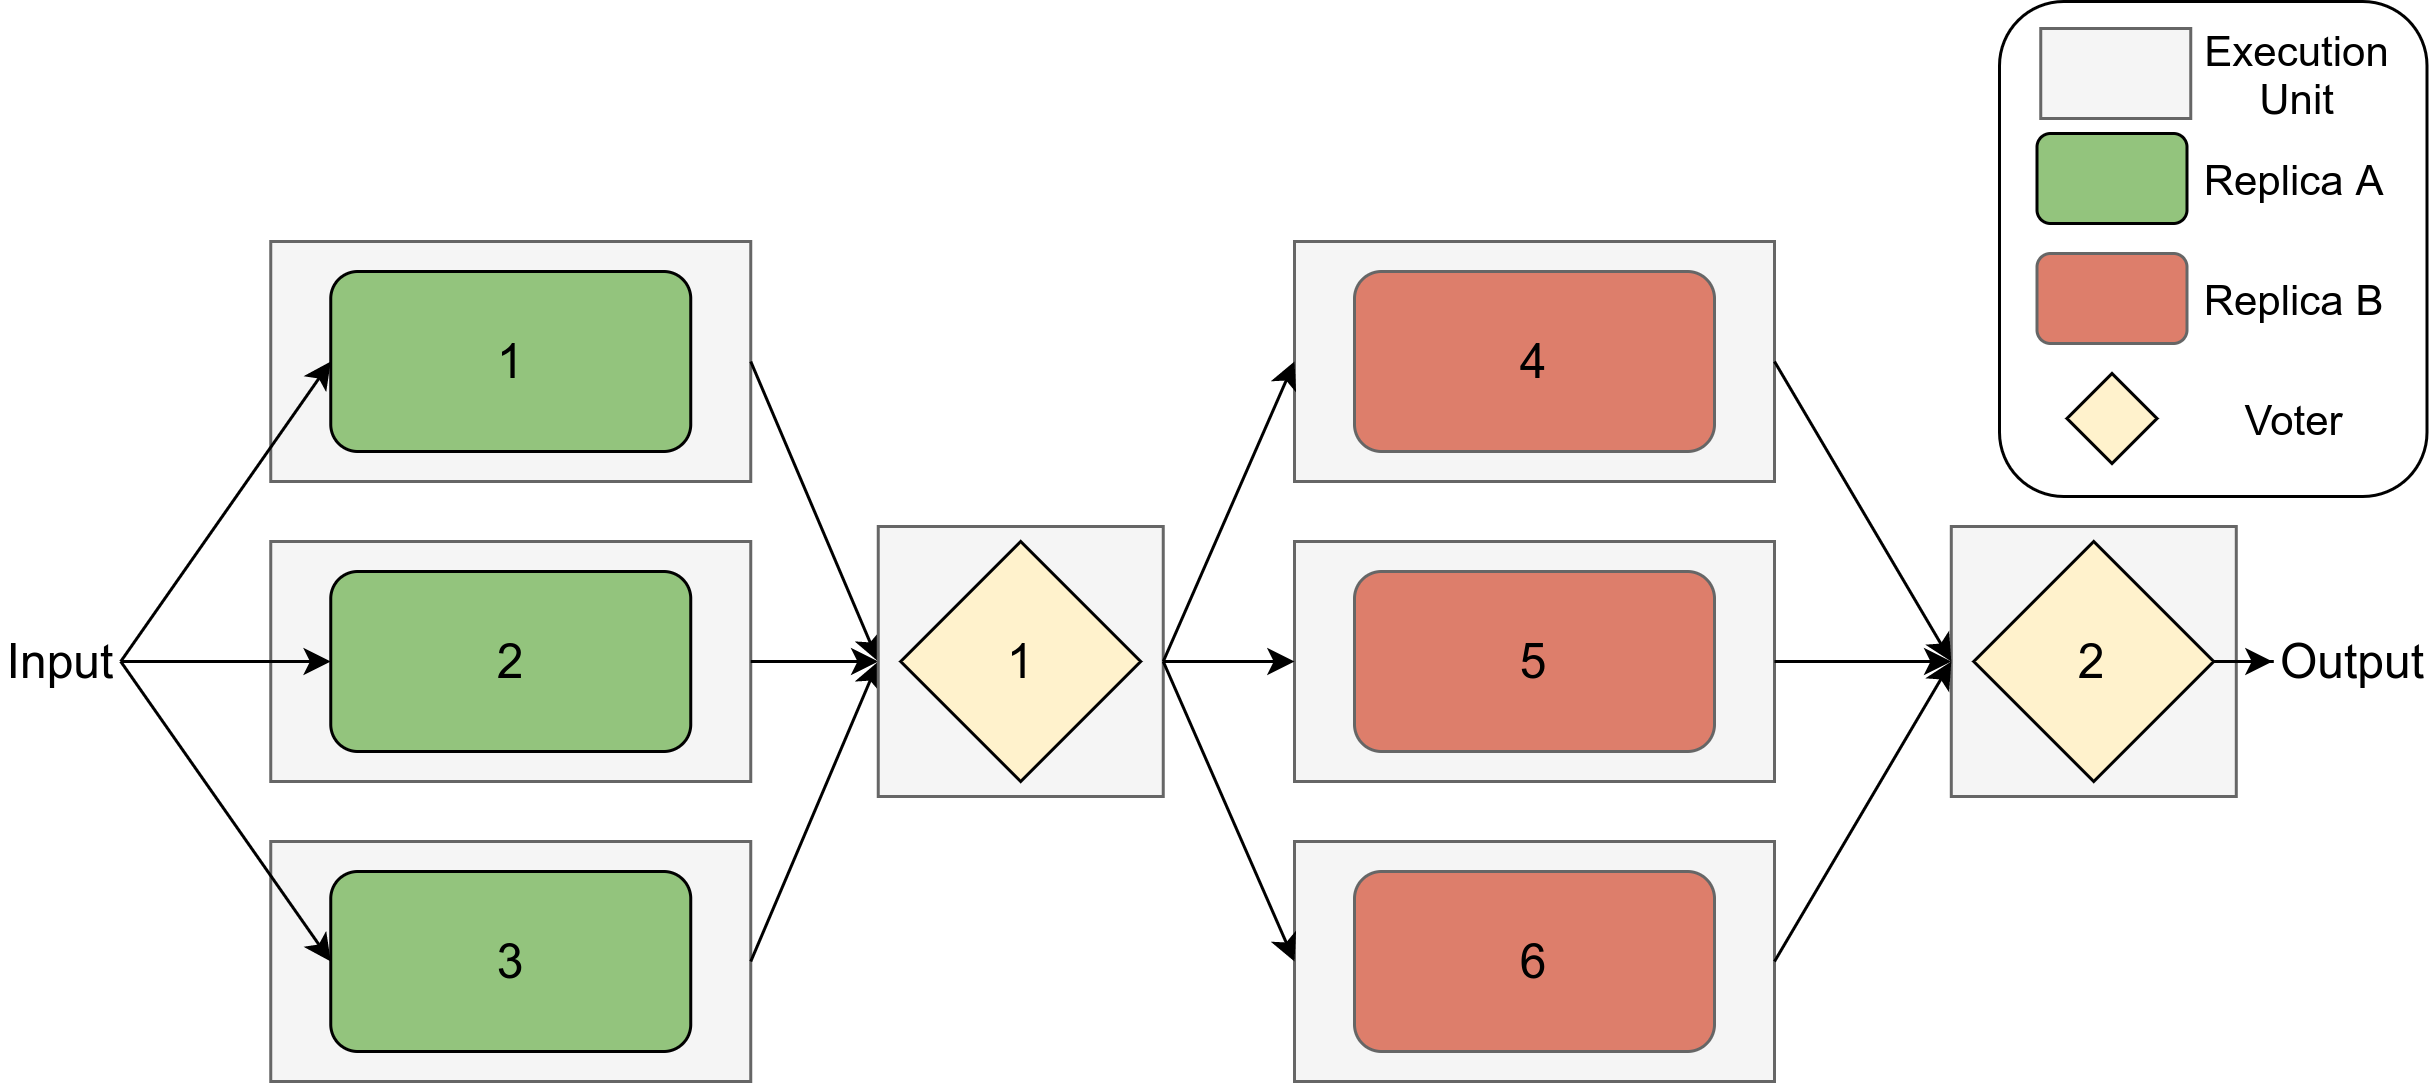
\includegraphics[width=0.9\linewidth]{images/IntermediateVoting}
	\caption{Intermediate voting mitigates the effect of individual computations on the final output. Therefore, voting is performed on provisional results before further processing. Another benefit of this approach is its pipelined fashion, which improves the overall system throughput. However, it also increases costs and communication overhead. }
	\label{fig:IntermediateVoting}
\end{figure}

\paragraph{Standby Redundancy}
\begin{figure}[!hb]
	\centering
	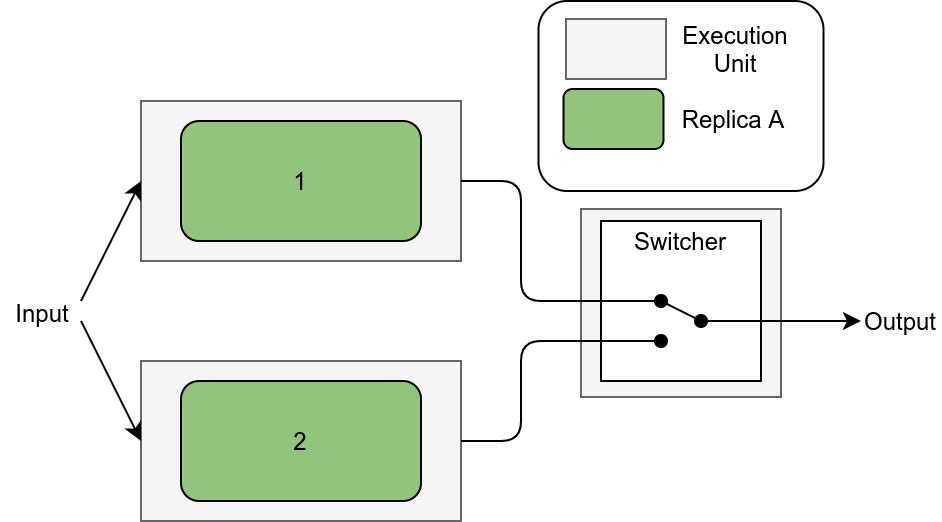
\includegraphics[width=0.8\linewidth]{images/ActiveSelectionRedundancy}
	\caption{With standby redundancy, a system can recover from individual component failures by replacing faulty components. Therefore, a switcher component performs error detection operations and delegates control over the output to the most trustworthy component.}
	\label{fig:StandbyRedundancy}
\end{figure}

As stated above, standby redundancy is an example of active hardware redundancy and builds on the concept of error detection, location, and recovery.
If an individual component experiences a fault, the resulting error and faulty component would need to be located so that the system can recover from the error by replacing the faulty component with a spare.
This concept is depicted in~\autoref{fig:StandbyRedundancy}, where two replicas are used, one as a primary and one as a secondary component.
A switching element observes the active component and, when no error is detected, provides control about the system's output to the active component.
As soon as the switching element detects an error, it excludes the active component from the system and transfers control about the system's output to the secondary component, which thereby becomes the active component.
When the secondary component is already running when the switching happens, this is called hot standby redundancy.
It is called cold standby redundancy when the secondary component needs to be turned on before being active.

\subsection{Software Redundancy}
One speaks of software redundancy when the redundancy concepts or error detection methods are implemented in software.
Examples for software redundancy are heartbeat messages to validate a component's accessibility, component-checking, or software voters.
In component-checking, a software or hardware program is used to monitor and validate a component's hardware, such as its memory, its clock, or its \gls*{CPU}.
A \abr{CPU}, for example, can apply redundant hardware for self-testing and fault-secureness~\cite{SelfCheckingProcessorDesign}.
While self-testing allows the detection of faults, self-secureness ensures that no fault can lead to an undetected error.
Thereby, it can be qualified whether a specific component's output can be considered valid or not.
This state is summarized into the term \texttt{internal consistency}.

\begin{definition}
A system or a component is said to be internally consistent, when any failure of this component is not based on a fault of its internal hardware.
Component checking mechanisms can determine a system's or component's internal consistency.
\end{definition}

By implication, when a system is internally consistent, any system failures can only be introduced by external causes - such as network delays, errors during data transmission, or defects in the inputs.

Further, voting or consensus algorithms can be implemented in software.
Similar to homogeneous and diverse hardware redundancy, diverse implementations of the same software can reduce the effect of faults in software.
The concept of diverse software programs is summarized under the term N-version programming, where a software program, which is based on the same specification, is developed by separate programmers~\cite{BarryFaultToleranceAnalysis}.

\subsection{Information and Time Redundancy}

\begin{figure}[!hb]
	\centering
	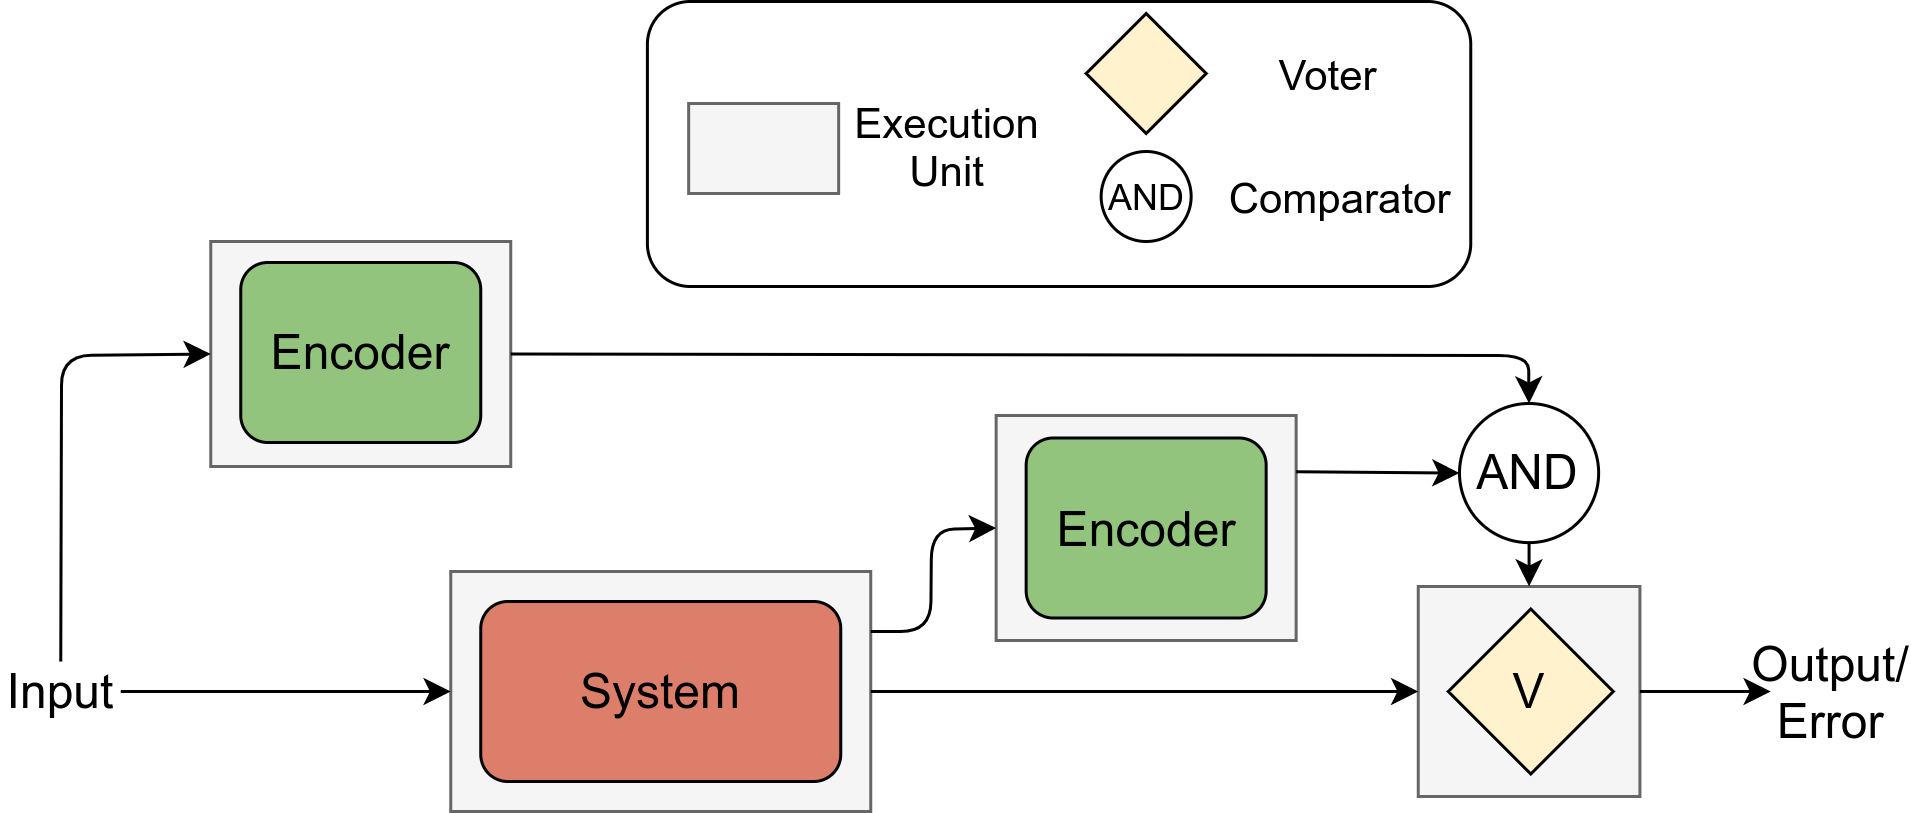
\includegraphics[width=0.8\linewidth]{images/ECC}
	\caption{\glsentryfull{ECC} applies both time and information redundancy. An encoder is used to encode both the input and output of a system (time redundancy). This encoded information is used in addition to the actual data (information redundancy). The encoder function needs to be chosen so that errors can be located and corrected~\cite{Su2005ECC}. An exemplary encoding that fulfills these characteristics are Hamming codes~\cite{HammingCodes}.}
	\label{fig:ECC}
\end{figure}

The addition of redundant information can allow the detection, masking, and recovery from faults~\cite{BarryFaultToleranceAnalysis}.
Examples for information redundancy include Hamming codes~\cite{HammingCodes}, checksums, or information duplication.
In Hamming codes, one or multiple parity bits are attached to the data bits to detect defects in the transmitted information.
Additionally, Hamming codes also allow to locate and correct errors in a bitstream.
Information- and time redundancy can be either implemented in software or in hardware using self-checking circuits.
John F. Wakerly argues that, when a system is non-transforming, the applied circuit is automatically self-checking~\cite{SelfCheckingProcessorDesign}.
He further compares different error-detection codes and provides self-checking hardware designs.
All information redundancy concepts share that they somehow encode redundancy into the transmitted data that can later be decoded.
\\

Another way of adding redundancy is to perform the same operation multiple times at different points in time.
This concept is called \texttt{Time Redundancy} and has the benefit that it does not necessarily require additional physical components.
Thereby, permanent faults in a system can be detected.

\autoref{fig:ECC} depicts an example of a combination of information and time redundancy using \gls*{ECC} techniques.
An encoder encodes the input and transmits this redundant information together with the input data.
After the system produces an output based on its input information, the output is also encoded and afterwards compared to the encoded input.
When there are anomalies between the system's input and its output, safety operations can be initiated.
The encoding function must be chosen so that it allows the detection of faults in the system.
In an exemplary case, where each input allows two possible outputs, the encoding function could generate two numbers for each input.
These two numbers are redundantly transmitted with the input.
The system's output is further encoded with the same encoding function, which generates an identification number for the generated output.
In a final step, it is verified whether the output's identification number corresponds with one of the input's two possible outputs.

\section{Related Work}
\paragraph{Redundancy to enhance Safety.}
Alapan Chakroborty demonstrates a development process of a reliable, safe, and fault-tolerant system using redundancy methods by an example of railway signaling~\cite{ChakrabortyFaultTolerantRailway}.
He argues that every fault-tolerant system needs to build upon real-time software solutions.
This requires both logical and timing correctness, which can only be achieved by correct redundancy management such as fault propagation, synchronization, and consensus among replicas.
At a fail-safe design's heart lies fault identification, masking and recovery.
Therefore, each redundant design should be subdivided into redundant elements not affected by any fault from outside the element.
Chakroborty calls these redundant elements \glspl*{FCR}.
As a second step, he proposes to define an interface between the \glspl*{FCR} so that they do not interfere with each other.
These two steps form a necessary precondition to predict the probability of failures in the system.

In order for the system to reduce redundant results to a single result and to mask failures, the concept of voting is demanded.
Voting, as Chakraborty claims, requires the \glspl*{FCR} to be in identical states, provide all redundant hardware with the same input, and perform identical real-time concurrent computations on each \gls*{FCR} for synchronization.
Finally, Chakraborty demonstrates the method by developing a railway signaling system.
\\

Bemment \etal evaluate redundancy concepts for railway track switching~\cite{BemmentEvaluationOfRedundancy}.
For this, they analyze and rate different hardware redundancy concepts and their combinations for railway networks.
Both reliability and cost estimations are made using mean time to failure caluculations and physical strain.
\\

An overview of possible hardware- and software redundancy concepts is provided by Barry W. Johnson \etal~\cite{BarryFaultToleranceAnalysis}.
He further made a cost, benefit, and performance analysis for each presented concept.
\\

In this work, the concepts proposed by Johnson \etal are extended based on the model by Chakraborty and by using and evaluating the feasibility of \gls*{DDS} for redundancy in the railway context.
While Chakroborty formulated demands and considerations for hardware- and software redundancy, Bemment \etal focussed on the design and evaluation of hardware redundant systems.
However, the evaluation approach of hardware according to the mean time to failure principle - used by Bemment \etal - can also be applied to software.
Typically, as Bemment \etal pointed out, an in-depth redundancy evaluation towards safety and reliability can only be made for well-defined use cases where hazards, risks and potential accidents are know.
Therefore, specific design decisions will be made throughout this thesis based on an \abr{ETCS} subset.
For further evaluations, an overview about possible accidents in railway is given by~\cite{ERTMSRailwayAccidents}.


\paragraph{Software development in the railway context.}
The CENELEC 50128 standard is a norm for software creating processes for railway applications so that the build software can be considered safe.
The 2011 version of CENELEC 50128, and resources needed to achieve a set level of assurance, are presented by Jean-Louis Boulanger~\cite{BoulangerStandards}.
Because software security - unlike hardware - is not affected by faulty components but by logic, it must be ensured separately.
First for building software for safety-critical railway applications, a risk analysis is made based on possible undesired events, their frequency, and risk level.
In addition, requirements and data structure are required before building software.
Then the development of the software can be started.
The software's correctness must be shown in subsequent tests.
\\

In this work, the system is developed based on an \abr{ETCS} subset.
The software is designed as a distributed and redundant system following the V-model.
Further, automatic integration and acceptance tests will be made to evaluate and approve the system's decisions.
Conducting and describing a detailed CENELEC 50128 conform design process for all software artifacts created in this thesis is outside its scope.
However, each software intended to be used in railway practice should pass the CENELEC 50128 norm.

\paragraph{\abr{DDS} in safety-critical systems.}
The \gls*{DDS} is already successfully deployed in distributed time- and safety-critical environments.
One example is given by Bijlsma \etal~\cite{DistributedSafety2020}, who extended the E-Gas layered monitoring concept to handle faults in a distributed and redundant system.
\Gls*{DDS} is applied to facilitate reliable communication among individual components in the system.
Their results can be used for automatic component checking mechanisms in a redundant system.
\\

Hadiwardoyo and Gao, who proposed the use of \gls*{DDS} in security cameras for subways as another example~\cite{DDSInSubways}.
They used \glspl*{QOS} to meet safety- and reliability requirements.
Results show that \abr{DDS} is suitable for scaling safety-critical systems where data is continuously transmitted in a dynamic and disruptive environment.
\\

Song \etal have proposed a system architecture that integrates the \abr{DDS} middleware into real-time embedded and safety-critical systems.
Thereby, they achieved a stable communication time~\cite{SongDDSInRealTimeSystems}.
Their approach has been verified by an \abr{UAV} combat scenario that operates in highly safety-critical scenarios.
Results have shown that the worst-case communication time for a one-kilobyte payload and a reliable communication \abr{QOS} is around 280 microseconds.
Since Song \etal exerted a topology that is similar to the one used in this work - namely a network switch with a 100~Mpbs Ethernet link for communication and external nodes - their findings can be seen as an affirmation for the approach used in this work.
However, they utilized a different \abr{DDS} implementation, so that their experiments need to be repeated in my case to approve their findings. 
\\

\begin{table}[h!]
	\begin{center}
		\caption{\abr{QOS} policies that affect the communication overhead (o) or the communication time (t). Each \abr{QOS} policy can either be applied to \texttt{DataWriters} (DR), \texttt{DataReaders} (DR), or \texttt{Topics} (T).}
		\label{tab:qos_garciavalls}
		\begin{tabularx}{\textwidth}{|l|l|X|}
			\hline
			\textbf{QoS policy} & \textbf{Entity} & \textbf{Description}\\
			\hline \hline
			Deadline (t) & DR \& DW & Maximal expected elapsed time between arriving data samples or instances. Maximal committed time to publish samples or instances.\\
			\hline
			Reliability (o) & DR \& DW & Global policy that specifies whether or not data will be delivered reliably. It can be configured on a per DataWriter/-DataReader connection. \\
			\hline
			History (o) & DR \& DW & Stores sent or received data in cache. It affects the Reliability \gls*{QOS} policy. \\
			\hline
			Resource Limits (o) & DP & Limit to the allocated memory. It limits the queue size for History when the Reliability protocol is used. \\
			\hline
			Latency Budget (t) & T \& DR \& DW & Indication on how to handle data that requires low latency. Allow specification of maximum acceptable delay from time the data is written to the time the data is received by the subscriber. \\
			\hline
			Time based Filter (t) & DR & Limits the number of data samples sent for each instance per a given time period. \\
			\hline
			Transport Priority (t) & DW & Establishes a given priority for the data sent by a writer.\\
			\hline
		\end{tabularx}
	\end{center}
\end{table}

A more general approach of how \gls*{DDS} can be used for enabling communication in distributed as well as time- and safety-critical environments is given by García-Valls \etal~\cite{GarciaVallsDDSInDistributed}.
They used a design of reading and monitoring sensor data to benchmark the middleware's communication performance with different \glspl*{QOS}.
One of their findings is a summary of \gls*{QOS}-policies that affect the system's communication overhead and communication time.
These are illustrated in~\autoref{tab:qos_garciavalls} and are especially important when examining real-time and mission-critical systems.
The results from García-Valls \etal show that the communication performance remains stable even under heavy load.
Even though they applied a different \gls*{DDS} implementation, the network topology and used hardware are comparable, which renders the results from García-Valls \etal useful for this work.

\paragraph{Time and availability for consensus based redundant systems.}
While redundant and distributed architectures are a typical approach to enhance a system's robustness, they also entail the demand to agree on certain data values.
Consensus algorithms are a way for components to coordinate and come to an agreement.
However, consensus algorithms also introduce a performance overhead, whose effects on the system's response time have been investigated by Sakic and Kellerer~\cite{SakicTimeInConsensus}.
Their studies focused on \abr{SDN} systems and \texttt{Raft}~\cite{RaftConsensusPaper}, a distributed consensus algorithm that takes care of data replication and leader election.
Results show that a system's response time in case of a random replica failing is linked to the probability of the leader being affected because this would entail a leader election process.
Eventually, in the studies from Sakic and Kellerer after one second, the cluster is almost guaranteed to deliver a response, even in the case of a random replica failing.
The situation looks different for combined correlated hardware and software failures.
Only around 20\% of the systems respond a result after one second when more than half of the replicas are affected.
In order to address this problem, Sakic and Kellerer propose a watchdog mechanism, which drastically increased the response probabilities in their experiments.
\\

Based on Sakic and Kellerer, the availability and response time for an actual system need to be evaluated in this work.
Further, the watchdog concepts should be kept in mind as it has a high impact on the system's response time in case of individual component failures.